\label{chap-intro}

This chapter introduces the topics that will be addressed in the next three chapters regarding finite area smoothing. The introduction proceeds as follows: first, \secref{intro-GAM} gives an introduction to smoothing using splines in two dimensions, \secref{intro-extending} then discusses the larger class of models to which the spatial smoothers belong, \secref{intro-inpractice} addresses some more practical issues, then finally \secref{intro-FAS} goes on to talk about existing approaches to spatial smoothing in a finite area.

\section{Smoothing in two dimensions using splines}
\label{intro-GAM}

In ecological studies, it is typical that one of the covariates collected is the location at which the sample has been taken. Two possible uses for such data are considered here. First, location may be the only covariate collected, in which case estimating the spatial distribution of the phenomena in question is the goal (usually by plotting some kind of surface as a function of geographical coordinates). Alternatively, the spatial covariates may be used to remove spatial autocorrelation from the data, making the effects of non-spatial covariates clear and this improving inferences.

The following two examples highlight these two different objectives:
\begin{enumerate}
\item The chlorophyl levels in the Aral sea are monitored using satellite images. Each pixel in the image represents an area of 9 kilometres square on the Earth. However, the satellite images are noisy and so adjacent pixels can have vastly different measured levels of chlorophyll. We would expect the levels to vary smoothly with location, so a model can be fitted to the image data which produces a smooth map of the chlorophyll concentration over the whole of the sea in an attempt to remove the noise. Figure \ref{aral-intro} shows both raw and smoothed chlorophyll levels in the Aral sea (this data is revisited in section \ref{aral-sec} and \ref{aral-revisit}).
\item We wish to model the distribution of the North sea whiting population through space and time. In particular numbers of fish of age one were recorded by pulling a net up through the water column at a set of sample points. The sample locations and dates were recorded along with sea surface temperature, the identity and nationality of the ship that took the measurement and the depth of the sea bed at the sample location. Such a model can be used to draw inference about how the population has changed over time (for example, to see if overfishing is a problem or perhaps to see if there are reporting discrepancies between ships). The whiting's distribution in space and time is non-homogeneous (in particular it is known that yearlings tend to be found close to the shore) and failing to model this spatial heterogeneity could introduce  bias in abundance estimates. Accurately modelling the spatial distribution is essential for reliable inference.
\end{enumerate}
In both of these examples it is assumed that the phenomena in question (chlorophyll concentration and whiting density) vary smoothly according to their spatial location in the sense that the underlying process does not jump around as location changes. In many situations this assumption is biologically plausible.

% Aral example
\begin{figure}[tb]
\centering
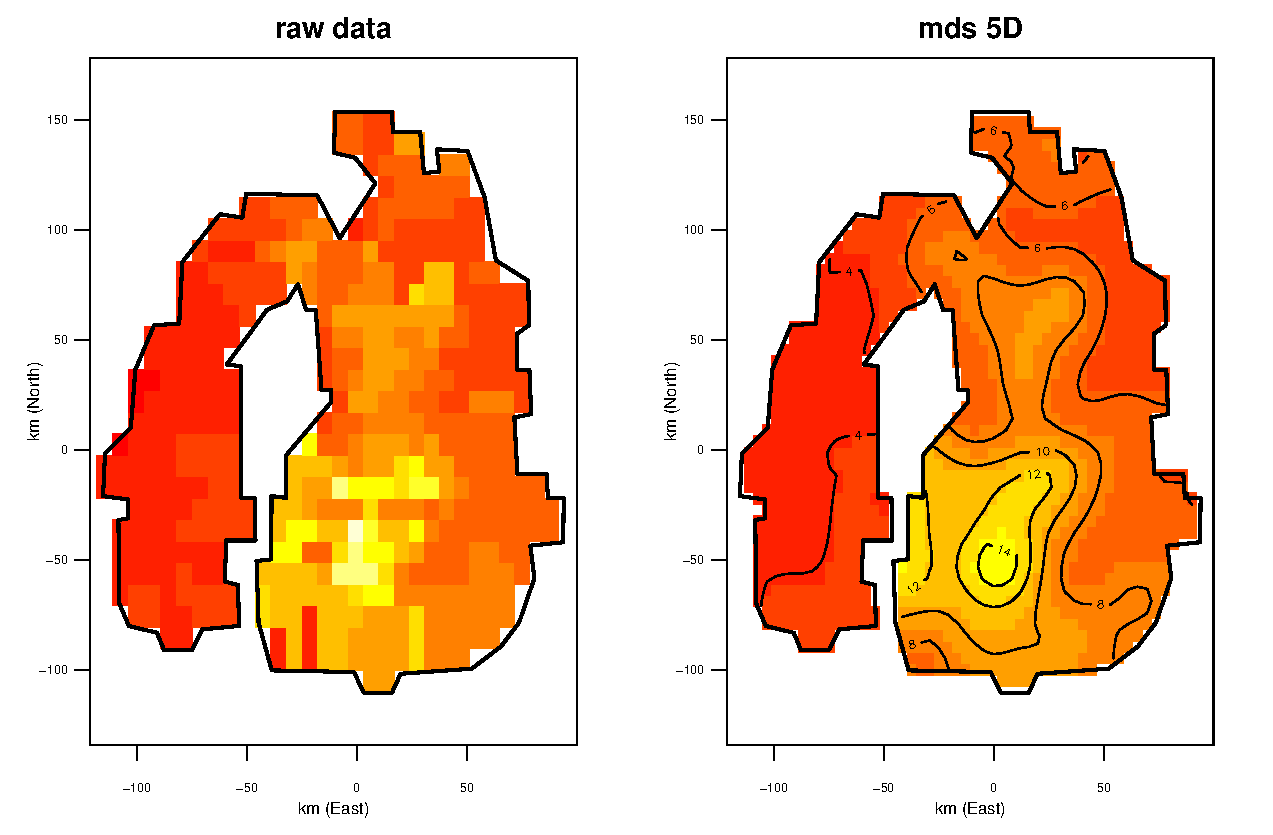
\includegraphics[width=4in, trim=0in 0in 0in 0.3in, clip]{mds/figs/aral-5d-duchon.pdf}\\
\caption{Left: raw chlorophyll levels in the Aral sea as recorded by the SeaWIFS satellite. Right: a smoothed version of the data. Further analysis of the data may be found in sections \ref{aral-sec} and \ref{aral-revisit}.}
\label{aral-intro}
\end{figure}

There are many ways to construct models for the data described in the above examples, popular methods include kriging (\cite{diggle},  \cite{schabenberger}), kernel density estimation (\cite{wandKDE}) and hierarchical Bayes models (\cite{banerjee}). Here the focus is on using \textit{splines} (e.g. \cite{wahba}) for spatial smoothing via \textit{additive models} (e.g. \cite{gammonograph}).

Of particular interest here are smooth functions of space, and since the models are additive the emphasis is on situations akin to example 1 above, since if a method can be used in this context, it can also be included in models like those in example 2, simply as an additive component. For this reason, non-spatial covariates are ignored (for now).

\subsection{Basic setup}
\label{intro-basic-setup}

First, denote observations of the phenomena of interest as $z_i$, where $i$ indexes the samples $i=1,\ldots,n$, if there are $n$ samples (in the examples above this would be the chlorophyll level or the yearling whiting catch at a particular point). Each  $z_i$ is the realisation of some random variable $Z_i$, where $Z_i=\mu_i+\epsilon_i$, where $\mu_i=\mathbb{E}[Z_i]$, the expected value of the $i^\text{th}$ observation. Here $\epsilon_i$ is an error term and is assumed to be normally distributed with zero mean and some variance, $\sigma^2$. The spatial coordinates of the sample are also recorded, denote them $\mathbf{x}_i = (x_{i1}, x_{i2})$ (coordinates could be measured in latitude and longitude, or as kilometres North and East of some reference point, known as Northings and Eastings). The objective is to model the expected value of the response ($\mu_i$) using the coordinates at which the data were collected.

We have assumed that the distribution of phenomena of interest varies smoothly in space, this is equivalent to saying that $\mu_i$ varies smoothly in space. If we let $f$ be some smooth function, then as $\mu_i = f(\mathbf{x}_i)$:
\begin{equation}
z_i = f(\mathbf{x}_i) + \epsilon_i.
\end{equation}
The observations are a sum of a smoothly varying spatial component and some random error. The problem is now how to estimate $f$.

One can imagine several possible ways of obtaining a suitable $f$, for example one might simply work through a large book of mathematical functions, tweaking parameters and hoping one would fit. Alternatively one might estimate $f$ as a kind of moving average of the values (for example LOESS, \cite{loess2}). The first option seems extremely time consuming (if it were even plausible) and the second will not give an ``explicit'' functional form at the end to slot into other procedures later. Rather than use either of these, a \textit{basis function} representation is used to form $f$. The idea is to build $f$ out of a sum of other known functions, ($b_j$s, say) scaled by coefficients ($\beta_k$, say) and then estimate these coefficients rather than the function as a whole. Mathematically:
\begin{equation}
 f(\mathbf{x}_{i}) = \sum_{j=1}^J \beta_j b_j(\mathbf{x}_{i}).
\label{intro-basisdecomp}
\end{equation}
Now some care must be taken in choosing both the form of the $b_j$s and how many are used ($J$) so that they give sufficiently flexible functions for $f$ over the whole of the domain that is to be smoothed over. 

The next few sections present a brief introduction to how spatial smoothing using splines works, with a particular emphasis on the spatial case. However, it should be noted that at all times the models presented can be extended to higher (and lower dimensions) and that two dimensions are used for clarity and relevance. The primary references for the rest of this section are \citeb{simonbook} and \citeb{rwc}, both provide excellent and complimentary introductions to the topic.

\subsection{Smoothing with penalties}
\label{GAMpenalties}

If $f$ is very flexible it is possible that in estimating the $\beta_j$s an $f$ which interpolates the data can be found. Interpolating the data is not useful since an $f$ that simply jumps from datum to datum does not say any more about the spatial distribution than merely looking at the data. To obtain an $f$ that interpolates the data, we can simply minimize the ordinary least squares (OLS) objective function. That is estimate the vector of coefficients, $\hat{\mathbf{\beta}}$, that minimizes:
\begin{equation}
\sum_{i=1}^n \left \{ z_i - f(\mathbf{x}_i) \right \}^2,
\label{intro-OLS}
\end{equation}
Given that $b_j$s are a sufficiently rich set of functions, this objective function does nothing to stop $f$ simply interpolating the data (which would give a value of 0 in the above expression). To stop this from happening the ``wigglyness'' of $f$ is penalized.

Penalizing the wigglyness (or \textit{roughness}, \cite{rwc}) of $f$ makes sense since (as stated above) the belief is that the underlying phenomena is smooth. Mathematically, taking (\ref{intro-OLS}) and adding on a penalty based on the wigglyness gives:
\begin{equation}
\sum_{i=1}^n \left \{ z_i - f(\mathbf{x}_i) \right \}^2 +  \lambda \int\int \lvert \lvert P f(\mathbf{x}) \rvert \rvert^2 \text{d}\mathbf{x}.
\label{intro-2d-objfcn}
\end{equation}
Here $P$ is some derivative operator, for example that might be the second derivatives (e.g. $P=\left ( \frac{\partial^2}{\partial x_1^2}, \sqrt{2} \frac{\partial^2}{\partial x_1 x_2}, \frac{\partial^2}{\partial x_2^2}\right )$ for the 2-dimensional case). The integrating the derivatives over the whole space gives a measure of the wigglyness of the function, functions which vary a lot will lead to large values of the integral and hence have larger penalties. The exact form of $P$ changes with the basis and dimensionality of the problem (as will be seen in the next section).

Depending on the situation, the penalty should have a different amount of influence on (\ref{intro-2d-objfcn}) and this is controlled by $\lambda$ ($\geq0$). The the \textit{smoothing parameter}, $\lambda$, controls the trade-off between interpolation (which happens as $\lambda \rightarrow 0$, leading to no penalty) and fitting a simpler function (which happens as $\lambda \rightarrow \infty$, where all terms are penalised aside from those for which the integral evaluates to zero: those in the \textit{nullspace} of the penalty). Figure \ref{lambda-ex} shows how different values of $\lambda$ effect the fitted smooth function. Determining the value of $\lambda$ will be covered in section \ref{GAMfitting}. For now it is assumed that some optimal $\lambda$ is known.

% example of setting lambda 
\begin{figure}[tb]
\centering
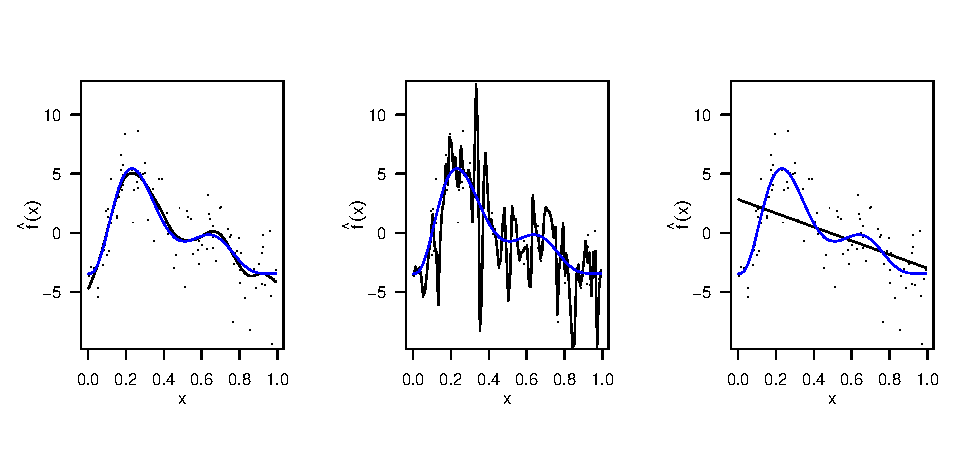
\includegraphics[width=6in]{intro/figs/lambda-ex.pdf}\\
\caption{An example of how different values of $\lambda$ effect the fitted smooth function of one variable. In the left panel, $\lambda$ is chosen optimally by GCV (see section \ref{GAMfitting}), in the middle panel the $\lambda=0$ giving an interpolating fit and in the right panel $\lambda=\infty$ leading to a straight line. In each panel the blue curve is the true function and the points are the data sampled from it with error.}
\label{lambda-ex}
\end{figure}

The expression for the penalty given in (\ref{intro-2d-objfcn}) looks like it might require a rather large amount of integration and that such a penalty would take a long time to compute however, it can be shown (\cite[p. 126]{simonbook}) that the integral can be written as:
\begin{equation}
\int\int \lvert \lvert P f(\mathbf{x}) \rvert \rvert^2 \text{d}\mathbf{x} = \bm{\beta}^\text{T} \mathbf{S} \bm{\beta},
\end{equation}
where the $ij^\text{th}$ element of $\mathbf{S}$ is the integral of the product of the appropriate derivatives (in the above example, second) of the $i^\text{th}$ and $j^\text{th}$ basis functions. Put more mathematically:
\begin{equation}
\mathbf{S}_{ij} = \int \int \left(P\mathbf{b}_{i}(\mathbf{x})\right ) \left (P\mathbf{b}_{j}(\mathbf{x}) \right )^\text{T}  \text{d}\mathbf{x}.
\label{pen-quadform}
\end{equation}
So in this case the penalty matrix $\mathbf{S}$ only needs to be computed once and so computation of the penalty is only a case of calculating the quadratic form in (\ref{pen-quadform}).

\subsection{Spline bases}

So far all that has been said about the form of $f$ is that it can be decomposed into a series of basis functions. Two bases are discussed here: \textit{thin plate regression splines} and \textit{P-splines}, which will be used in this thesis.

\subsubsection{Thin plate regression splines}
\label{GAMtprs}
\label{GAMtprspenalty}

In (\ref{intro-basisdecomp}) $f$ was decomposed into a sum of basis functions. For a \textit{thin plate spline} (\cite{duchon77}), this summation is split into two parts: a set of global polynomials that act over the whole of the data and a set of \textit{radial basis functions}, one centered at each datum. One can think of this as a global trend (in the 2-dimensional case, linear functions of the two coordinates) with extra flexibility provided by the radial basis functions.

The thin plate spline basis is:
\begin{equation}
f(\mathbf{x}) = \sum_{i=1}^n \delta_i \eta_{m,d}(r_i) + \sum_{j=1}^M \alpha_j \phi_j(\mathbf{x}),
\label{tprs-basis} 
\end{equation}
where $r_i=\lvert \lvert \mathbf{x}-\mathbf{x_i}\rvert \rvert$ (the Euclidean norm of $ \mathbf{x}-\mathbf{x_i}$) and the radial basis functions $\eta_{m,d}(r)$ are defined as:
\begin{align*}
\eta_{m,d}(r) =\begin{cases} \frac{(-1)^{m+1+d/2}}{2^{2m-1}\pi^{d/2}(m-1)!(m-d/2)!} r^{2m-d} \log(r) &\quad{\text{$d$ even,}}\\
\frac{\Gamma(d/2-m)}{2^{2m}\pi^{d/2}(m-1)!} r^{2m-d} &\quad{\text{$d$ odd.}}
\end{cases}
\end{align*}
where $m$ is the \textit{derivative order} (e.g. $m=2$ so far), $d$ is the dimension of the smooth (i.e. the dimension of $\mathbf{x}$, 2 in a spatial setting) and $\Gamma$ is the gamma function. The $\phi_j$s are $M=\left( \begin{smallmatrix} m+d-1 \\ d  \end{smallmatrix}\right)$ linearly independent polynomials of degree less than $m$ which span the space of polynomials in $\mathbb{R}^d$; all of the $\phi_j$s therefore lie in the nullspace of the penalty and are therefore unpenalized.

The thin plate spline penalty is given as:
\begin{equation}
J_{m,d} = \int \ldots \int_{\mathbb{R}^d} \sum_{\nu_1 + \dots + \nu_d=m} \frac{m!}{\nu_1! \dots \nu_d!} \left ( \frac{\partial^m f(x_1,\dots,x_d)}{\partial x_1^{\nu_1} \ldots  \partial x_d^{\nu_d}} \right )^2 \text{d} x_1 \ldots  \text{d} x_d,
\label{tprs-pen}
\end{equation}
where $m$ and $d$ are as above and the summation and $\nu_1,\ldots,\nu_d$ terms simply ensure that derivatives are taken with respect to all the parameters in all of the necessary combinations. It is also important to note that to maintain continuity in $f$, $2m>d$. This all looks rather complex, however in the 2-dimensional case, (\ref{tprs-pen}) looks much simpler, as shall be seen below. An important feature of the thin plate spline penalty is that it treats all of the directions of the smoother equally; e.g. wigglyness in the $x_1$ direction has the same weight in the penalty as in the $x_2$ direction (and so on in higher dimensions). This property is known as \textit{isotropy} and is usually appropriate in a spatial setting, since there is nothing special about one geographical coordinate over another when it comes to the smoothness of the function to be fitted.

Putting the above into the 2-dimensional spatial smoothing case and setting the penalty order to be $2$ ($d=2$ and $m=2$), we have:
\begin{equation*}
f(\mathbf{x}) = \sum_{i=1}^n \delta_i \eta_{2,2}(r_i) + \sum_{j=1}^3 \alpha_j \phi_j(\mathbf{x}),
\end{equation*}
where:
\begin{equation*}
\eta_{2,2}(r) = \frac{1}{8\pi} r^2 \log(r).
\end{equation*}
and the penalty in (\ref{tprs-pen}) is then:
\begin{equation*}
J_{2,2} = \int \int \left ( \frac{\partial^2 f(x_1,x_2)}{\partial x_1^2} \right )^2 + 2\left ( \frac{\partial^2 f(x_1,x_2)}{\partial x_1  \partial x_2} \right )^2 + \left ( \frac{\partial^2 f(x_1,x_2)}{\partial x_2^2} \right )^2 \text{d} x_1 \text{d} x_2.
\end{equation*}
The nullspace of the penalty consists of three functions: $\phi_1(\mathbf{x})=1, \phi_2(\mathbf{x})=x_1 \text{ and } \phi_3(\mathbf{x})=x_2$, which make no contribution to $J_{2,2}$. Figure \ref{tprs-basis-fig} shows some examples of 2-dimensional thin plate basis functions.


% tprs basis fig
\begin{figure}[p]
\centering
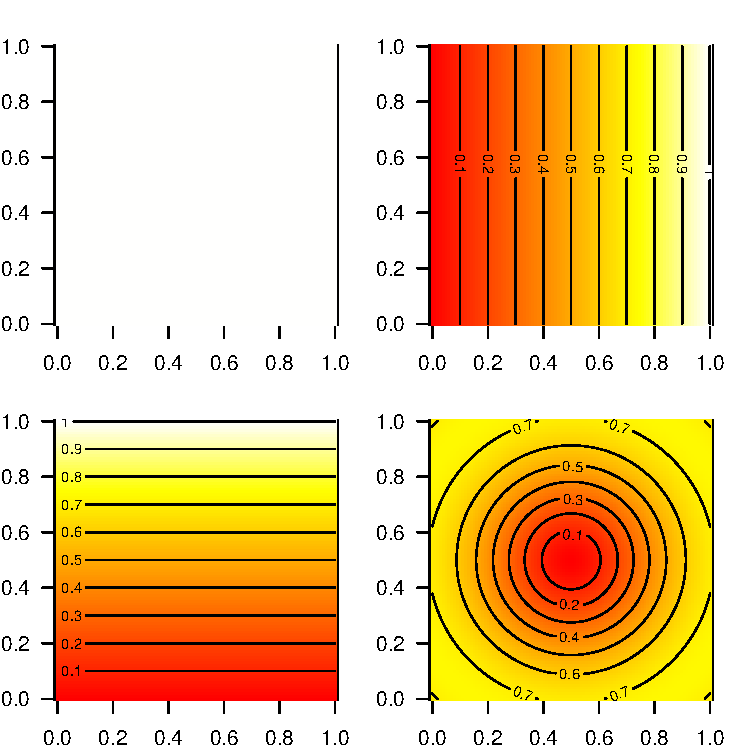
\includegraphics[width=\textwidth]{intro/figs/tprsex.pdf}\\
\caption{Example of a thin plate spline basis. The first three are $\phi_1(\mathbf{x})=1, \phi_2(\mathbf{x})=x_1 \text{ and } \phi_3(\mathbf{x})=x_2$, which are in the nullspace of the $J_{2,2}$ penalty. The bottom right plot shows an example of a radial basis function centred on $(0.5,0.5)$.}
\label{tprs-basis-fig}
\end{figure}

With one radial function per datum the computational time taken to both evaluate and fit the model is very large and runs the risk of being too complex in many situations since the number of parameters is so big. To avoid this problem, one could either ($i$) select (perhaps randomly) some of the data and use only those points to create the basis and then use the full data to fit the model (i.e. changing the index of the summation in the first term of (\ref{tprs-basis})) or ($ii$) select a (relatively small) representative set of points within the space covered by the data (though not necessarily data locations) which would be evenly spread out enough to create the basis (changing the $\mathbf{x}_i$s in the first summation in (\ref{tprs-basis}) -- these points are known as \textit{knots}). Both approaches have potential problems, namely: how many points should be chosen and where they should best be located.

Both of the above approaches effectively reduce the size of the basis (changing the limit on the first summation in (\ref{tprs-basis})), however both methods do this in a fairly arbitrary way. There is no objective measure of whether the points selected are ``good''. Say we put the evaluations of the radial basis functions in a ($n \times n$) matrix $\mathbf{E}$ such that the $ij^\text{th}$ element of the matrix is the $j^\text{th}$ basis function evaluated at the $i^\text{th}$ datum (i.e. $\mathbf{E} = \eta_{m,d}\left (\vert\vert\mathbf{x}_i - \mathbf{x}_j \vert\vert \right )$), reducing the computations required to fit the model can be achieved by reducing the rank of $\mathbf{E}$. In the previous two approaches the rank reduction was performed by removing columns from $\mathbf{E}$ (randomly sampling the data) or changing the number of columns by changing the location of the evaluations (using knots). 

One way of reducing the size of $\mathbf{E}$ is by performing an eigen-decomposition (so $\mathbf{E}=\mathbf{U}\mathbf{\Lambda}\mathbf{U}^\text{T}$, where the columns of $\mathbf{U}$ are orthogonal eigenvectors and $\mathbf{\Lambda}$ is a diagonal matrix of eigenvalues decreasing in absolute value down the diagonal). Picking the $k$ largest eigenvalues and truncating at that point (taking the first $k$ columns of $\mathbf{U}$ and the top right $k\times k$ submatrix of $\mathbf{\Lambda}$) gives $\mathbf{E}_k(=\mathbf{U}_k\mathbf{\Lambda}_k\mathbf{U}_k^\text{T})$. It can be shown that the reduced rank matrix $\mathbf{E}_k$ gives the best approximation to $\mathbf{E}$ (see \cite{wood2003} for details). In practise, $k$ is set to be ``large enough'' and further reduction in basis complexity is performed by penalization (see \secref{GAMEDF}).

\subsubsection{P-splines}
\label{intro-psplines}

P-splines (\cite{eilersmarx96}) consist of B-spline basis function with discrete penalties, so before thinking about P-splines, the properties of B-splines are considered. B-splines are simple local basis functions; they are simple in that they all have the same shape and local in that they only have an effect near where they are centred (at the knots) -- \textit{compact support}. Taking (\ref{intro-basisdecomp}), we replace the $b_j$s with an $(m+1)^\text{th}$ order B-spline $B_j^m$ (where the order is chosen). Note that the $B_j^m$s are only a function of one covariate, $x_{i1}$s, at this point but will be expanded to higher dimensions below. So, the basis representation of $f$ given in (\ref{intro-basisdecomp}) becomes:
\begin{equation*}
f_{x_1}(x_{1i}) = \sum_{j=1}^{J+m+1} \beta_j B^m_j(x_{1i}).
\end{equation*}
The $B_j^m$s are defined recursively as:
\begin{equation*}
B_j^m(x) = \frac{x-x^*_j}{x^*_{j+m+1} - x^*_j} B_j^{m-1}(x) + \frac{x^*_{j+m+2} -x}{x^*_{j+m+2} - x^*_{i+1}} B_{j+1}^{m-1}(x) \quad \text{for } i=1,\ldots,J,
\end{equation*}
and
\begin{equation*}
 B_j^{-1}(x)=\begin{cases}
1 \quad x_j \leq x < x_{j+1}\\
0 \quad \text{otherwise}. 
\end{cases}
\end{equation*}
The $J+m+1$ knots $x^*_j$ are evenly spaced over the $x$-axis and these, along with the order of the basis, determine how flexible $f$ is. Each $B^m_j(x)$ is non-zero over the $m+3$ adjacent knots. Contrary to their rather complex functional form, the functions shown in figure \ref{bs-basis} are rather simple. From left to right the panels show B-splines bases with $m=1,2,3$ for evenly spaced knots over $(0,1)$.

% b-splines example 
\begin{figure}[tb]
\centering
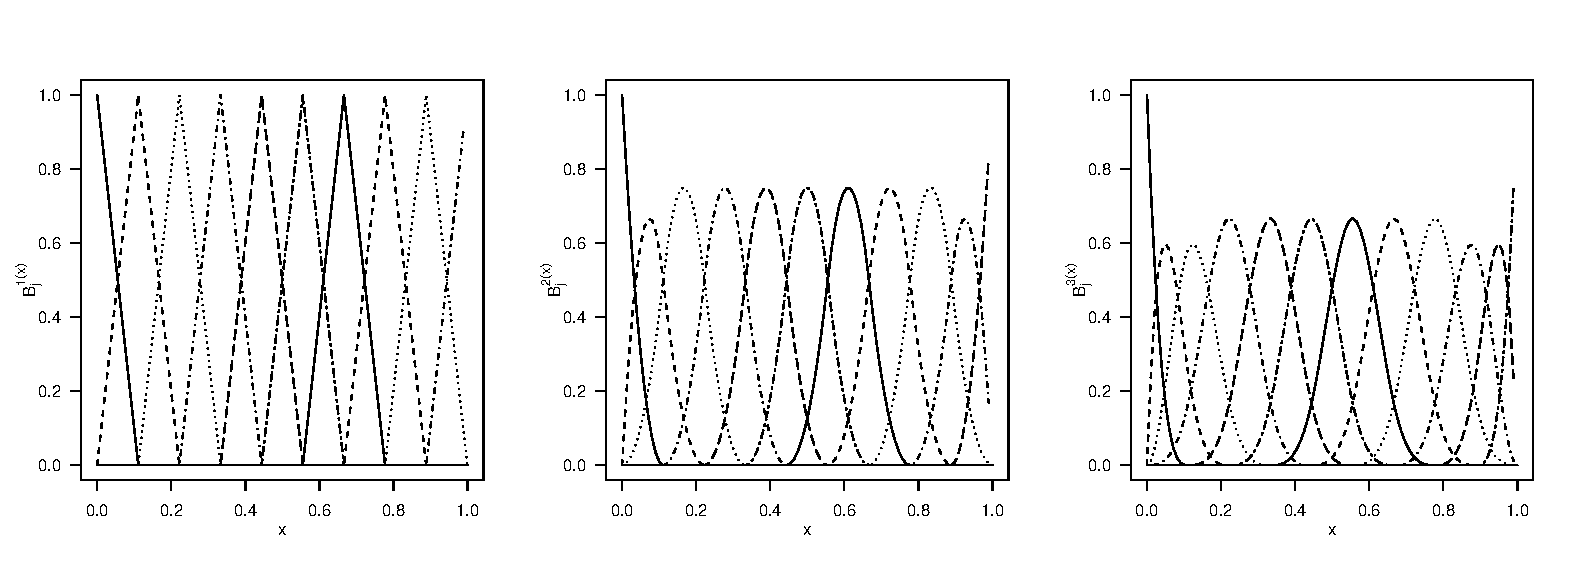
\includegraphics[width=\textwidth]{intro/figs/bspline-ex.pdf}\\
\caption{An example of B-spline basis functions for $m=1, 2$ and $3$ (from left to right) with evenly spaced knots (these are located at the peaks of the basis functions).}
\label{bs-basis}
% generated by phd-smoothing/thesis/intro/figs/bspline-ex.R 
\end{figure}

P-splines take the B-spline basis and add a penalty structure. Because of their local nature, the penalty is somewhat different to the general penalty in (\ref{intro-2d-objfcn}) and is based on finite differences. The idea is that smoothness only needs to be enforced on neighbouring basis functions (since the $B^m_j$s are defined locally) so (\ref{intro-2d-objfcn}) becomes:
\begin{equation*}
\sum_{i=1}^n \left \{ z_i - f_{x_1}(x_{1i}) \right \}^2 +  \lambda \sum_{j=1}^{J+m+1} \Delta^2 \beta_j,
\end{equation*}
where $\Delta^2 \beta_j = \beta_j -2\beta_{j-1} + \beta_{j-2}$ (the second difference). Such a penalty is very fast to compute, since it can be found directly from the coefficients.

\subsubsection{Tensor products}
\label{GAMtensor}

P-splines are defined only in one dimension, however, it is possible to build 2-dimensional (and higher) smooths from \textit{tensor products} of 1-dimensional smooths. This is made possible by thinking of each 1-dimensional basis as a marginal of a higher dimensional smooth. A spatial smooth of, say $x_1$ and $x_2$ can be constructed by first writing down the basis expansions for the marginal smooths of $x_1$ and $x_2$ (in general terms, since this applies to all splines not just P-splines):
\begin{equation*}
f_{x_1}(x_1) = \sum_{j=1}^J \beta_j b_j(x_{1}), \quad  f_{x_2}(x_2) = \sum_{j=1}^J \delta_j d_j(x_{2}).
\end{equation*}
where the $\delta_j$ and $d_j$ are analogous to $\beta_j$ and $b_j$ and assuming that the basis size $J$ is the same for each direction (though this need not be the case). To make $f_{x_1}$ vary with $x_2$ we can then simply make the $\beta_j$s a function of $x_2$, the simplest way of doing this would be to define:
\begin{equation*}
\beta_j(x_2) = \sum_{j=1}^J \delta_j d_j(x_{2}).
\end{equation*}
so then $f_{x_1,x_2}$ would is defined as:
\begin{equation*}
f_{x_1, x_2}(x_1) = \sum_{j=1}^J \sum_{j=1}^J \delta_j d_j(x_{2}) b_j(x_{1}).
\end{equation*}
Finally, there is now one penalty for each direction yielding:
\begin{equation*}
\lambda_{x_1} \int\int \left \{P_{x_1} f_{x_1, x_2}(x_1,x_2)\right \}^2 \text{d}x_1\text{d}x_1 + \lambda_{x_2} \int\int \left \{P_{x_2} f_{x_1, x_2}(x_1,x_2)\right \}^2 \text{d}x_1\text{d}x_1,
\end{equation*}
where $P_{x_1}$ and $P_{x_2}$ are derivative operators with respect to $x_1$ and $x_2$ respectively (or could be replaced by two P-spline penalties). 

Although only a very simplistic example is given here, tensor product splines provide an extremely useful tool, allowing for extra dimensions to be added to models using different bases. The use of a different smoothing parameter for each direction allows for \textit{anisotropic} smoothing, so that covariates that are measured on different scales (for example temperature and length) may be combined into one tensor product smooth, avoiding the assumption that the degree of smoothing required is the same in both directions. In particular this can be useful when constructing a spatiotemporal smooth: for example using a thin plate spline for the spatial part of the smooth (so the spatial part of the model is isotropic) then taking a tensor product of that with a P-spline basis (or another 1-dimensional thin plate spline) for the temporal effect (so a different amount of smoothing can be used for each direction).

\subsection{Fitting}
\label{GAMfitting}

Turning attention to estimating $\bm{\hat{\beta}}$ and $\hat{\lambda}$ (or $\hat{\bm{\lambda}}$ in the tensor product case), a simple and effective way to find optimal values is to assess how well the model performs on data which was not in the sample -- i.e. assessing the prediction error of the model. The \textit{ordinary cross validation} (OCV) score does exactly this by fitting the model to all but one of the datum and calculating the difference between the prediction of the excluded datum and its true value. Rather than fitting $n$ models to the data (one for each excluded datum), the \textit{generalized cross validation} (GCV) score can be used, which can be written as follows, allowing for easy computation:
\begin{equation}
\mathcal{V}_g = \frac{n \lvert\lvert \mathbf{z} - \mathbf{\hat{f}}(\mathbf{x})\rvert \rvert^2}{\left \{n-\text{tr}(\mathbf{A}) \right \}^2},
\label{intro-GCV}
\end{equation}
where $\mathbf{A}$ is the hat (or influence) matrix for the smoother (see \secref{GAMEDF}) and $\text{tr}(\mathbf{A})$ indicates the trace of $\mathbf{A}$. Numerical minimization of $\mathcal{V}_g$ gives the parameters ($\bm{\hat{\beta}}$ and $\hat{\lambda}$) which minimize the prediction error of the model. Further details are given in \citeb[pp.  134-137]{simonbook}. 



\section{Extending to more complex models}
\label{intro-extending}

So far only smooths of two geographical coordinates with normal errors in the response have been discussed. This section gives an overview of some of the extensions to the models discussed above.

\subsection{Higher dimensional smooths}

Although in the above, the focus has been on including on geographical coordinates as explanatory variables, other covariates (or combinations of covariates) can be included in an additive way. The notation in (\ref{intro-2d-objfcn}) and (\ref{pen-quadform}) is simply extended in this case and all of the above results hold, simply by defining $f(\mathbf{x})=\sum_k f_k(\mathbf{x}^{(k)})$ for smooths $f_k$ of corresponding covariates ($\mathbf{x}^{(k)}$) and the smoother matrix $\mathbf{S}$ is replaced by $\mathbf{S}= \sum_k \lambda_k \mathbf{S}_k$ where, rather than only having one smoothing parameter ($\lambda$), there are many smoothing parameters ($\lambda_k$). With such additive models identifiability becomes an issue since each of the $f_k$ can only be found up to some additive constant (since one could add a value, $a$ to $f_1$, say and then subtract it from $f_2$ leading to the same model as if $a$ were not included. To get around this problem \textit{identifiability constraints} are used to ensure that the models are identifiable: ensuring that the sum of the values of each function at the observed values is zero (for linear functions this means that the function passes through the origin). As seen in the thin plate spline case, the order of the penalty can be changed (and, indeed, is required to change) according to the number of dimensions that smoothing takes place in. Ensuring that the derivative order in the penalty is high enough to prevent overly complex functions being unpenalized is essential. Smoothing in high dimensions can be unreliable and numerically tricky but not impossible (as will be seen later in chapter \ref{chap-gds}).

\subsection{Generalized additive models}
\label{intro-extending-gams}

Other exponential family error distributions may be used in place of normal errors. If other exponential family error distributions are used, we call this a \textit{generalized} additive model (GAM)  and in that case we may model $\eta_i=g(\mu_i)$ where $g$ is a \textit{link function} (in the same sense as the GLM case, see \cite[p. 8]{GEEbook}) and $\eta_i$ is the linear predictor. A more complex fitting routine must then be used to estimate the parameters. The ``hierarchical'' optimisation method of \citeb{remlpaper} is used here. That is: at each iteration a smoothing parameter is selected to optimize the GCV score, this $\lambda$ then implies a set of model coefficients (the best $\bm{\beta}$ for that given $\lambda$) which are found using PIRLS (see below), the algorithm then proposes a new value of $\lambda$ based on the derivatives of $\mathcal{V}_g$ with respect to $\log \lambda$ at this point. This continues until convergence.

Thinking of the GAM as a penalized GLM means the PIRLS algorithm can be used to find $\bm{\hat{\beta}}$. Consider first the usual GLM model matrix $\mathbf{X}$. By appending the basis evaluations of each datum as columns of $\mathbf{X}$ (i.e. $\mathbf{X}:=\left ( \mathbf{X},\mathbf{X}^* \right )$, where the $ij^\text{th}$ element of $\mathbf{X}^*$ is  $b_j(\mathbf{x}_i)$), the smooth terms in the model can be included in the usual model matrix setup. The PIRLS algorithm is as follows (\cite[p. 138]{simonbook}):

First define $\eta_i = \mathbf{X}_i\bm{\beta}$ (where $\mathbf{X}_i$ is the $i^\text{th}$ row of $\mathbf{X}$) as the linear predictor such that $\mu_i = g^{-1}(\eta_i)$ and the variance function, $V(\mu^{[k]})$, such that $\text{Var}\left ( Z_i \right ) = \phi V(\mu^{[k]})$ ($\phi$ is the scale parameter, see \cite[p. 62]{simonbook}). At iteration $k$ the PIRLS algorithm is:
\begin{enumerate}
\item Given the current linear predictor estimate and mean response vectors ($\bm{\eta}^{[k]}$ and $\bm{\mu}^{[k]}$, respectively) calculate the diagonal weight matrix with the following elements:
\begin{equation*}
\mathbf{W}^{[k]}_{ii}  \propto \frac{1}{V(\mu_i^{[k]})g^\prime(\mu_i^{[k]})^2},
\end{equation*}
and the pseudodata:
\begin{equation*}
s_i = g^\prime(\mu_i^{[k]})^2(z_i-\mu_i^{[k]}) + \mathbf{X}_i\bm{\beta}^{[k]},
\end{equation*}
stored in the $n$-vector $\mathbf{s}$. $g^\prime(\mu_i^{[k]})$ is the first derivative of the link function with respect to $\mu_i^{[k]}$.
\item Minimize
\begin{equation*}
\lvert \lvert \sqrt{\mathbf{W}^{[k]}} (\mathbf{s}^{[k]} - \mathbf{X}\bm{\beta})  \rvert \rvert^2 + \lambda \int\int P^2 f(\mathbf{x}) \text{d}\mathbf{x}
\end{equation*}
with respect to $\bm{\beta}$, giving $\bm{\beta}^{[k]}$ and hence allowing the calculation of $\bm{\eta}^{[k]}$ and $\bm{\mu}^{[k]}$.
\end{enumerate}
This procedure is iterated to convergence of $\bm{\beta}$ for the given smoothing parameter(s). Further information on PIRLS in the GLM context can be found in chapter 1 of \citeb{GEEbook}.

\subsubsection{Other GAM fitting methods}

It has been observed (\cite{reissogden}) that GCV can sometimes have problems with multiple minima (i.e. the optimisation can get stuck at a non-optimal $\lambda$). An alternative to minimizing the GCV score is to use a likelihood-based method such as approximate REML or ML, which does not suffer from this problem (\cite{remlpaper}). The key to understanding restricted maximum likelihood or (marginal) maximum likelihood methods is the realisation that the estimates of the coefficients (the $\bm{\hat{\beta}}$) are the posterior modes of the distribution of $\bm{\beta}|\mathbf{z}$ if $\bm{\beta} \sim N(\mathbf{0},\mathbf{S}^-)$ (where $\mathbf{S}^-$ the generalized matrix inverse of $\mathbf{S}$). When the $\bm{\beta}$ are considered to be random variables, smoothing parameters can then be thought of as variance parameters and a likelihood can then be formed (this is known as the \textit{random effects formulation}).  This likelihood can then be optimized with respect to $\lambda$ in the same hierarchical way as with GCV above. At each iteration the optimal $\bm{\beta}$ is found via PIRLS.

\citeb[pp. 120-123]{rwc} provide an interesting discussion of automatic smoothing parameter selection. In particular they note that as the number of data increases ($n\rightarrow\infty$), GCV only slowly converges to finding the optimum smoothing parameter, this leads to the variability of the smoothing parameter to be quite high. In general GCV tends to select more complicated functions than likelihood based methods leading to overfitting to the data (see \cite{remlpaper} and \cite{reissogden}). REML and ML on the other hand will tend to fit smoother functions. However, it is important to note that this is a manifestation of the variance--bias trade-off. GCV will lead to less biased but more variable fits whereas likelihood based methods will be less variable but more biased. It does not seem that there is a clear ``best'' method for selecting smoothness but rather that both methods are imperfect in different ways. These issues did not manifest themselves when performing the spatial smoothing, but there were hints of this happening in the non-spatial models (see \secref{gds-examples}).

There are many other ways of fitting GAMs, such as backfitting (\cite{gammonograph}, see also \secref{gds-intro}), Markov chain Monte Carlo (MCMC, e.g. \cite{fahrmeir2004}) or integrated nested Laplace approximations (INLA, \cite{inla}). The methods described above were chosen over these methods for several reasons. Backfitting and MCMC are quite computationally expensive, especially when larger models are used (see \cite{simonbook}, pp. 213-215 for why this is the case for backfitting). MCMC-type approaches can be improved by exploiting sparse bases (like P-splines) however, thin plate splines (and their nice properties like isotropy) cannot be used. INLA can be very fast, however when many terms are included it becomes computationally expensive (\cite{inla} suggest more than 10 become problematic).

\cite{ruppertreview} gives an overview of developments in the area of semiparametric regression in general during the 2003--2007 period.

\section{Smoothing in practice}
\label{intro-inpractice}

This final section deals with two topics not covered above: assessing model performance and the practical implementation of the methods detailed above.

\subsection{Mean squared error}

Simulation studies will be used extensively to evaluate the proposed methods. In order to make such evaluations, some metric must be chosen. Mean squared error (MSE) is a standard approach to assessing the performance of a model, in terms of prediction error. The MSE of the fitted model $\hat{f}$ is defined as:
\begin{equation*}
\text{MSE}(\hat{f}) = \mathbb{E}\left [\left \{ \hat{f}(X) - f(X) \right \}^2 \right ],
\end{equation*}
which (if there are $n_p$ prediction points) can be calculated as:
\begin{equation}
\widehat{\text{MSE}}(\hat{f}) = \frac{1}{n_p} \sum_{i=1}^{n_p} \left \{\hat{f}(\mathbf{x}_i) - f(\mathbf{x}_i) \right \}^2,
\label{DEFN-MSE}
\end{equation}
where $f(\mathbf{x}_i)$ is the ``true'' values of $f$ at the prediction points, $\mathbf{x}_i$.  It makes sense for $\mathbf{x}_i$ not to be the data since an $\hat{f}$ that simply interpolates will have zero MSE, but may still be a very bad model for the unobserved locations. When MSE is mentioned from now on, it will be with reference to $\widehat{\text{MSE}}$ in (\ref{DEFN-MSE}).

To test to see if models' MSEs are significantly different, the Wilcoxon signed paired rank test is used in analysing the results from simulations.

\subsection{The Brier score}
\label{DEFN-brier}

The Brier score (\cite{brier50}) is useful when the response variable is binary (a more general version of the score for $n$-ary variables can also be used). In this case the probability of observations belonging to a particular class (0 or 1 in the binary case) is measured, so it makes sense to assess the model performance using the probabilities rather than just the classifications. The score is similar in form to the MSE:
\begin{equation}
\text{BS} = \frac{1}{n_p} \sum_{i=1}^{n_p} \left \{\hat{f}_p(\mathbf{x}_i)-f(\mathbf{x}_i) \right \}^2
\end{equation}
where subscript $f_p$ indicates that the predictions are on the probability scale, rather than the prediction on the response scale. The Brier score has the advantage of offering a more granular measure of the model errors, since probabilities will be continuous on $(0,1)$ rather than dichotomous (or $n$-chotomous) class predictions.

\subsection{Effective degrees of freedom}
\label{GAMEDF}

The hat or influence matrix, $\mathbf{A}$, is the matrix such that $\hat{\bm{\mu}} = \mathbf{A}\mathbf{z}$. It has the rather useful property that taking the trace of $\mathbf{A}$ ($\text{tr}(\mathbf{A})$) gives the \textit{effective degrees of freedom} (EDF) of the model. The EDF gives an measure of the complexity of the fitted model. The higher the EDF, the more complex the model. The EDF can be a useful tool when it comes to model choice and model diagnostics; if models seem to have similar performance then looking at the EDF may give a reason to choose one over another (if one is simpler), or if models are overly complex (but cannot simply be plotted).

Since the models used here are penalised, it is the penalty term that controls the overall wigglyness of the spline and hence the EDF. If there was no penalty then the value of the EDF would be the number of elements of $\bm{\beta}$ (minus any identifiability constraints, see above). In most cases the basis dimension is set as an upper bound, the smoothing penalty suppresses parts of the model. Therefore basis dimension is not a major concern provided that it is not set too low (\cite[p. 161]{simonbook}). 

\subsection{Leave-one-out cross validation}
\label{DEFN-LOOCV}

When analysing non-simulated data (where the true values are unknown) it is still sometimes necessary to quantify the out-of-sample error in predictions. This can be achieved using leave-one-out cross validation (LOOCV). The LOOCV score is calculated as:
\begin{equation}
\text{LOOCV} = \frac{1}{n} \sum_{i=1}^n \left \{ \hat{f}^{-i}(\mathbf{x}_i) - z_i \right\}^2,
\end{equation}
where $\hat{f}^{-i}$ is the model fit to all of the data except the $i^\text{th}$, so one can think of the LOOCV score as a measure of fit to unseen data.

\subsection{Fitting GAMs using \texttt{mgcv}}
\label{intro-mgcv}

Throughout this this thesis the software package \texttt{mgcv} by Simon Wood is used. The package is free (GPL) software for the language \textsf{R} (\cite{Rsoftware}). The library gives a simple, extensible collection of fitting routines, bases and diagnostics.


\subsection{Summing up}

This section has hopefully given a brief introduction to generalized additive models in the setting of spatial smoothing. The next section goes into the particulars of the problem that will be address in the first three chapters of the thesis: finite area smoothing.


\section{Finite area smoothing}
\label{intro-FAS}

\subsection{Overview of finite area smoothing}

As we have seen in the previous section, splines are a popular way of performing spatial smoothing in two dimensions. To recap, a typical application in ecological modelling consists of a response modelled as a function of its spatial coordinates. The estimated function can then be used to perform inference on the population, whether that be an abundance estimate, density map or as part of a larger model, taking into account nuisance spatial effects. Finite area smoothing concerns the situation in which the domain over which this smoothing takes place is bounded.

When the geographical region has a \emph{complex boundary}, features from one part of the domain can unduly influence other parts. Considering the boundary as a polygon, a complex boundary is a non-convex polygon, in particular when the non-convexity is relatively extreme. Often this consists of having some peninsula-like feature(s) in the domain with notably different observation values on either side of the feature. Given that there is some scientific motivation as to why those parts of the domain should not affect each other, features such as peninsulae give rise to a phenomenon known as \emph{leakage}.

Leakage occurs when a smoother inappropriately links two pats of a domain (\cite{soap}). The phenomenon is problematic since it causes the fitted surface to be mis-estimated; this can then lead to incorrect inference (e.g. bias), which is clearly not desirable. Leakage can be seen in \fig{leakage} where the high values in the upper half of the domain leak across the gap to the lower values below and vice versa.

% leakage example 
\begin{figure}
\centering
% trim order l b r t
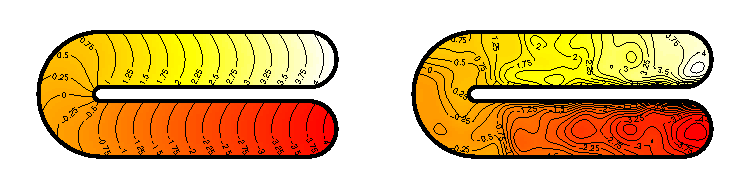
\includegraphics{intro/figs/ramsay-leak.pdf}\\
\caption{An example of leakage. A thin plate regression spline was fit to data sampled from the function on the left, the model smooths across the gap in the middle of the domain (right.)}
\label{leakage}
\end{figure}

The problem of leakage arises because of the way in which the smoother measures how near objects are to one another. Most smoothing techniques use the Euclidean metric to measure the distance between data. Clearly though, this approach is a flawed: biological populations do not conform to Euclidean geometry in their movement patterns and hence their observed positions will reflect this. Just as whales no not uniformly distribute themselves across sea and glacier, fish do not lay their eggs on land. Natural and man-made barriers carve up the landscape (and seascape), partitioning biological populations; spatial models should take this into account.

The distribution of the population may be smooth, just not necessarily over $\mathbb{R}^2$ (\cite{wangranalli}). Modelling the structure of the domain correctly by embedding the extra information relating to the shape of the boundary (whether this be implicitly or explicitly) allows for more accurate inference.

\subsection{Ramsay's horseshoe function as a benchmark for finite area smoothing}

\label{ramsayfunc}

\citeb{ramsay} proposes a function which can be used to benchmark new approaches to 2-dimensional smoothing. The function takes the form of a horseshoe shape which is flat across the domain has a gradient along the domain's major axis. This can be seen in \fig{orig-fs}. \citeb{soap} modifies the test function by adding curvature across the minor axis of the shape. This was added in order to avoid the horseshoe function lying in the nullspace of their model's penalty, making the problem too easy for the method. It is the second shape that will be used for simulations here and shall be referred to as the \emph{Ramsay horseshoe} throughout; it is shown in \fig{leakage}.

% original horseshoe from Ramsay's paper
\begin{figure}
\centering
% trim order l b r t
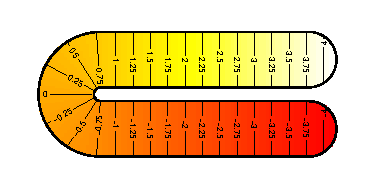
\includegraphics{intro/figs/orig-fs.pdf}\\
\caption{The horseshoe function as it appeared in \citeb{ramsay}.}
\label{orig-fs}
\end{figure}

As mentioned above, when the smoothing problem is specified in terms of Euclidean distance, the model takes the distance between the points in the two arms of the horseshoe as the distance over the gap in-between them, rather than the distance along the major axis of the shape. This causes the high function values from one side to contaminate the other side (and the low to contaminate the high).
		
\subsection{Previous approaches to leakage}
\label{intro-leakageapproaches}

The cause of leakage can be characterised in two ways: either the smooth does not respect the boundary of the domain, or the smooth does not take into account the geometry of the domain (in particular with regard to the distance between points within the domain). Previous work in this area has been to combat leakage along these two lines. Work of \citeb{ramsay} and \citeb{soap} both use a partial differential equation (PDE) boundary condition approach to try to prevent leakage, where as \citeb{wangranalli} and \citeb{eilerstalk} modify the way that inter-point distances are measured in order to avoid smoothing across boundaries. These four main works may be summarised as follows:

\begin{enumerate}
\item \citeb{ramsay} proposes finite element $L$-splines (FELSPLINEs). The $L$-spline replaces the usual penalty term (see \secref{GAMpenalties}) with:
\be
\int \int_\Gamma (L_p f)^2 \text{d}x_1\text{d}x_2,
\ee
where $\Gamma$ is the domain in question and $L_p$ is a roughness operator defined as:
\be
L_p=\Delta^p+c_{p-1}\Delta^{p-1}+\dots+c_1\Delta+c_0I.
\ee
Here $I$ is the identity operator, the $(c_0,\dots, c_p)$ are constants and the $\Delta$ is the Laplacian (sum of second derivatives with respect to $x_1$ and $x_2$). Although any differential operator could be used for $L_p$, the Laplacian gives rise to a set of polynomials which are isotropic.

In order to find the minimiser of the objective function formed by using this penalty in place of the one in (\ref{intro-2d-objfcn}), Ramsay takes a finite element approach. First he triangulates the domain, then he constructs a set of bivariate quadratic polynomial basis functions over each triangle, specifying that there be continuity over the edges of the triangles. By taking the FELSPLINE objective function and transforming it into a variational form (in the same way as a PDE is), the approximation to the minimiser of the objective function is found. 

Since the triangulation and hence the penalty of the FELSPLINE is only calculated over the domain, and the continuity is specified over neighbouring cells, the method prevents leakage. However, although FELSPLINE does not exhibit leakage on the original horseshoe (as in \fig{orig-fs}), in practice the model makes unrealistic physical assumptions. The boundary conditions of FELSPLINE specify that the gradient is zero, along normals to the boundary. This is not always physically realistic. \citeb{soap} show that by using a different response function for the horseshoe shape (see \secref{sc-alt-horsehoe}), the FELSPLINE performance begins to falter.

FELSPLINE does not offer a realistic physical model and is therefore not a viable solution to the finite area smoothing problem in general.

\item \citeb{wangranalli} adopt a ``within-area distance'' formulation for thin plate splines. They choose to use the geodesic distance between two points, that being the shortest path within the domain. This gives a definition of how near objects are in the domain. This is then used as the distance in the radial basis functions of a \tprs, rather than using the usual Euclidean distance (see \secref{GAMtprs}).

Wang and Ranalli first create the complete weighted, undirected graph ($G$, say) with a data point at each vertex and the distance between each pair of vertices as the weights on the edges. They then find the restricted graph of $G$, $G_k$, in which each vertex is only connected to its $k$ nearest neighbours. With this new, restricted graph the geodesic distances between each pair of vertices can be calculated using Floyd's algorithm (\citeb{Floyd}).

As the authors point out, the quality of the approximation is dependent on the size of the data set and its density. At low densities the estimated geodesic distance will tend towards the Euclidean, at high densities the approximation tends, asymptotically toward the true geodesic distance (\citeb{bernstein}). Even if  dense enough data were available, the method will be rather slow since Floyd's algorithm is cubic in the number of vertices (the size of the data set). 

Taking these points into account, Wang and Ranalli's approach appears cumbersome, slow and dependent on dense data.

\item The soap film smoother (\cite{soap}) uses a rather simple physical model to prevent leakage from occurring. First, consider the domain boundary to be made of wire, then dip this wire into a bucket of soapy water, you will then have (provided it doesn't pop(!)) a soap film in the shape of your boundary. Consider the wire to lie in the $x_1-x_2$ plane and the height of the soap film at a given point to be the functional value of the model (i.e. in the $z$ direction). This film is then distorted smoothly by moving it toward the data, while minimising the surface tension in the film.

Mathematically, the soap film smoother is constructed by first specifying a set of functions $\rho_k(x,y)$, which are each solutions to the Laplace equation in two dimensions:
\be
\frac{\partial^2\rho}{\partial x_1^2} + \frac{\partial^2\rho}{\partial x_2^2} = 0
\ee
except at one of the knots ($x^*_{1k},x^*_{2k}$). Then, solving Poisson's equation in 2-dimensions:
\be
\frac{\partial^2 g_k}{\partial x_1^2} + \frac{\partial^2 g_k}{\partial x_2^2} = \rho
\label{soap-poisson}
\ee
with $\rho=\rho_k(x_1,x_2)$, where $k$ indexes the knots and the boundary condition $\rho=0$. The set of basis functions for the soap film smoother, $g_k(x_1,x_2)$ is found, along with $a(x_1,x_2)$ (the solutions to \eqn{soap-poisson} when $\rho=0$, subject to the boundary condition). These bases are then summed to form:
\be
f(x_1,x_2)=a(x_1,x_2)+\sum_{k=1}^n \gamma_k g_k(x_1,x_2),
\ee
the soap film smoother, where the $\gamma_k$ are parameters to be estimated. The (isotropic) penalty term (\secref{GAMpenalties}) is:
\be
\int_\Gamma \left (\frac{\partial^2 f}{\partial x_1^2}+\frac{\partial^2 f}{\partial x_2^2} \right )^2\text{d}x_1\text{d}x_2,
\ee
Differing from the standard \tprs\ penalty since: (\emph{i}) the integration occurs only over $\Gamma$, (\emph{ii}) there is no mixed derivative term, and (\emph{iii}) the whole integrand is squared rather than each term individually. This allows the $x_1$ and $x_2$ term's derivatives to be traded off against each other so the nullspace of the penalty is infinite dimensional. This allows those functions in the nullspace to be sufficiently wiggly to meet any boundary conditions.

The solution of the PDEs above, yielding the basis and penalty, is the most computationally expensive part of the procedure. Knots to use for $x_{1k}^*$ and $x_{2k}^*$ must be specified, usually using a grid. Numerical problems occur when knots are placed in boundary cells in the PDE solution grid.

Although mathematically elegant, the soap film smoother is a rather complex model. It also treats the boundary differently from the interior and uses a cyclic spline in order to approximate the boundary values. This treatment of the boundary seems rather unnatural and it may not always be physically realistic to consider the boundary in such a way.

Soap film smoothers are available in the \textsf{R} package \texttt{soap}, which is an extension to \texttt{mgcv}.

\item An alternative approach to treating the boundary as something special is to transform the space in which the points lie to instead lie in a different domain which is more suitable for smoothing. For example, with Ramsay's horseshoe, it seems intuitive to simply bend the horseshoe into a long strip and then smooth on that domain.

Indeed, \citeb{eilerstalk} proposed using the \sch\ transform for this very purpose (the author independently came to the idea in 2008). Using the \sch\ transform for smoothing will be elaborated on in chapter \ref{chap-sc}, so only a brief summary is given here.

The basic idea is to find a function, $\varphi$ say, that takes points in the domain the data lie in ($W$, say) and maps them to a domain ($W^*$, say) in which smoothing is easier ($\varphi : W \mapsto W^*$, mathematically).

Creating some kind of mapping between the space in which the data lies and the space in which conventional smoothers perform well is convenient. Relying on existing, tested methodology is clearly appealing. This approach also benefits from not treating the boundary as a special in the basis setup.
\end{enumerate}

Outside of the smoothing spline and GAM literature methods have also been suggested, in particular, when using a kriging approach (see \cite[pp. 425-430]{MASS} for a concise introduction, \cite{schabenberger} or \cite{diggle} for a thorough treatment). Kriging consists of modelling the spatial correlation between points via the \textit{semivariogram} and a spatial trend via a mean function (similar to the linear predictor in the smoothing case, although there are flavours of kriging where the mean is considered constant and/or known). Semivariogram models assume that the correlation between points is related to the distance between the points but not their position (this is known as \textit{stationarity}, and comes in varying degrees, \cite[pp. 42-44]{schabenberger}). Although not specifically designed to deal with leakage issues (although leakage will manifest itself as a breakdown of stationarity in a kriging context), several authors have suggested the use of some kind of transformation of the data points in space in order to maintain stationarity by approximating within-area distances with equivalent Euclidean distances  via multidimensional scaling (\cite{mdskrig}, \cite{crabkrig}, \cite{curriero}). This is similar to the methods proposed in chapters  \ref{chap-mds} and \ref{chap-gds}. A comparison between these geostatistical methods and those proposed in this thesis is given in \secref{gds-krig}, once the proposed methods have been fully explained.

Chapters \ref{chap-sc}, \ref{chap-mds} and \ref{chap-gds} investigate the combination a transformation of space and conventional smoothers to solve the problem of leakage in finite area smoothing.
